% sinc 函数
% 函数|连续|积分

\pentry{连续函数\upref{contin}}

$\sinc$ 函数的定义为
\begin{equation}
\sinc x = 
\leftgroup{
&\frac{\sin x}{x} &\quad & (x \ne 0)\\
&\quad 1 && (x = 0)
}\end{equation}

$\sinc$ 函数的图像如\autoref{sinc_fig1}, 可以证明, 该函数在 $x=0$ 处是连续的, 即
\begin{equation}
\lim_{x \to 0}\frac{\sin x}{x} = \sinc 0 = 1
\end{equation}

\begin{figure}[ht]
\centering
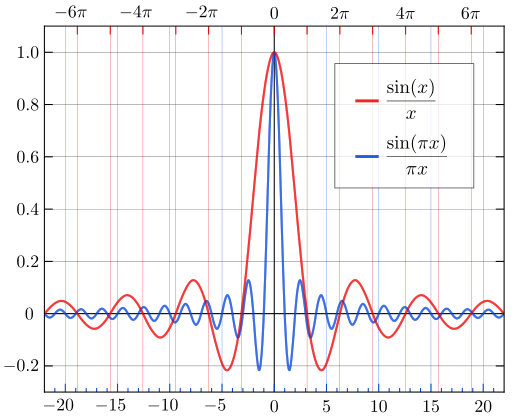
\includegraphics[width=10cm]{./figures/sinc1.png}
\caption{sinc 函数(来自维基百科)} \label{sinc_fig1}
\end{figure}

归一化积分
\begin{equation}
\int_{-\infty}^{+\infty} \sinc^2(x) \dd{x} = \pi
\end{equation}
